\subsection{VT Detection Algorithm}
\label{sec:svtvt}
%The limited sensing resolution and noise in the \ac{EGM} signals make it is impossible for the device to achieve 100\% accuracy for SVT/VT discrimination.
Device companies have developed different algorithmic components to distinguish \ac{SVT} from \ac{VT}, referred to as \emph{discriminators}. 
Each discriminator utilizes the history of timing and/or morphology of the EGM signals to determine whether the current rhythm is a \ac{VT} or \ac{SVT} (or neither).
%The decisions of each discriminators are then combined using a decision tree structure to decide whether to deliver or inhibit therapy.
No single discriminator is sufficient on its own to discriminate between \ac{SVT} and \ac{VT}, because these classes of arrhythmias can appear similar in a number of criteria.
Therefore discriminators are organized in a decision tree.%, as illustrated in Fig. \ref{fig:BS_det}.
We have implemented the detection algorithms Rhythm ID from Boston Scientific and PRL+W from Medtronic. 
This section gives an overview of both algorithms.

%We will need the following definition: an \emph{interval} is the amount of time between two consecutive electrical events. 
%Thus a ventricular interval is the duration between two ventricular events.
%Intervals are variable in length. 
%Consistently short intervals imply a fast rhythm.

\begin{figure*}[t]
	\centering
	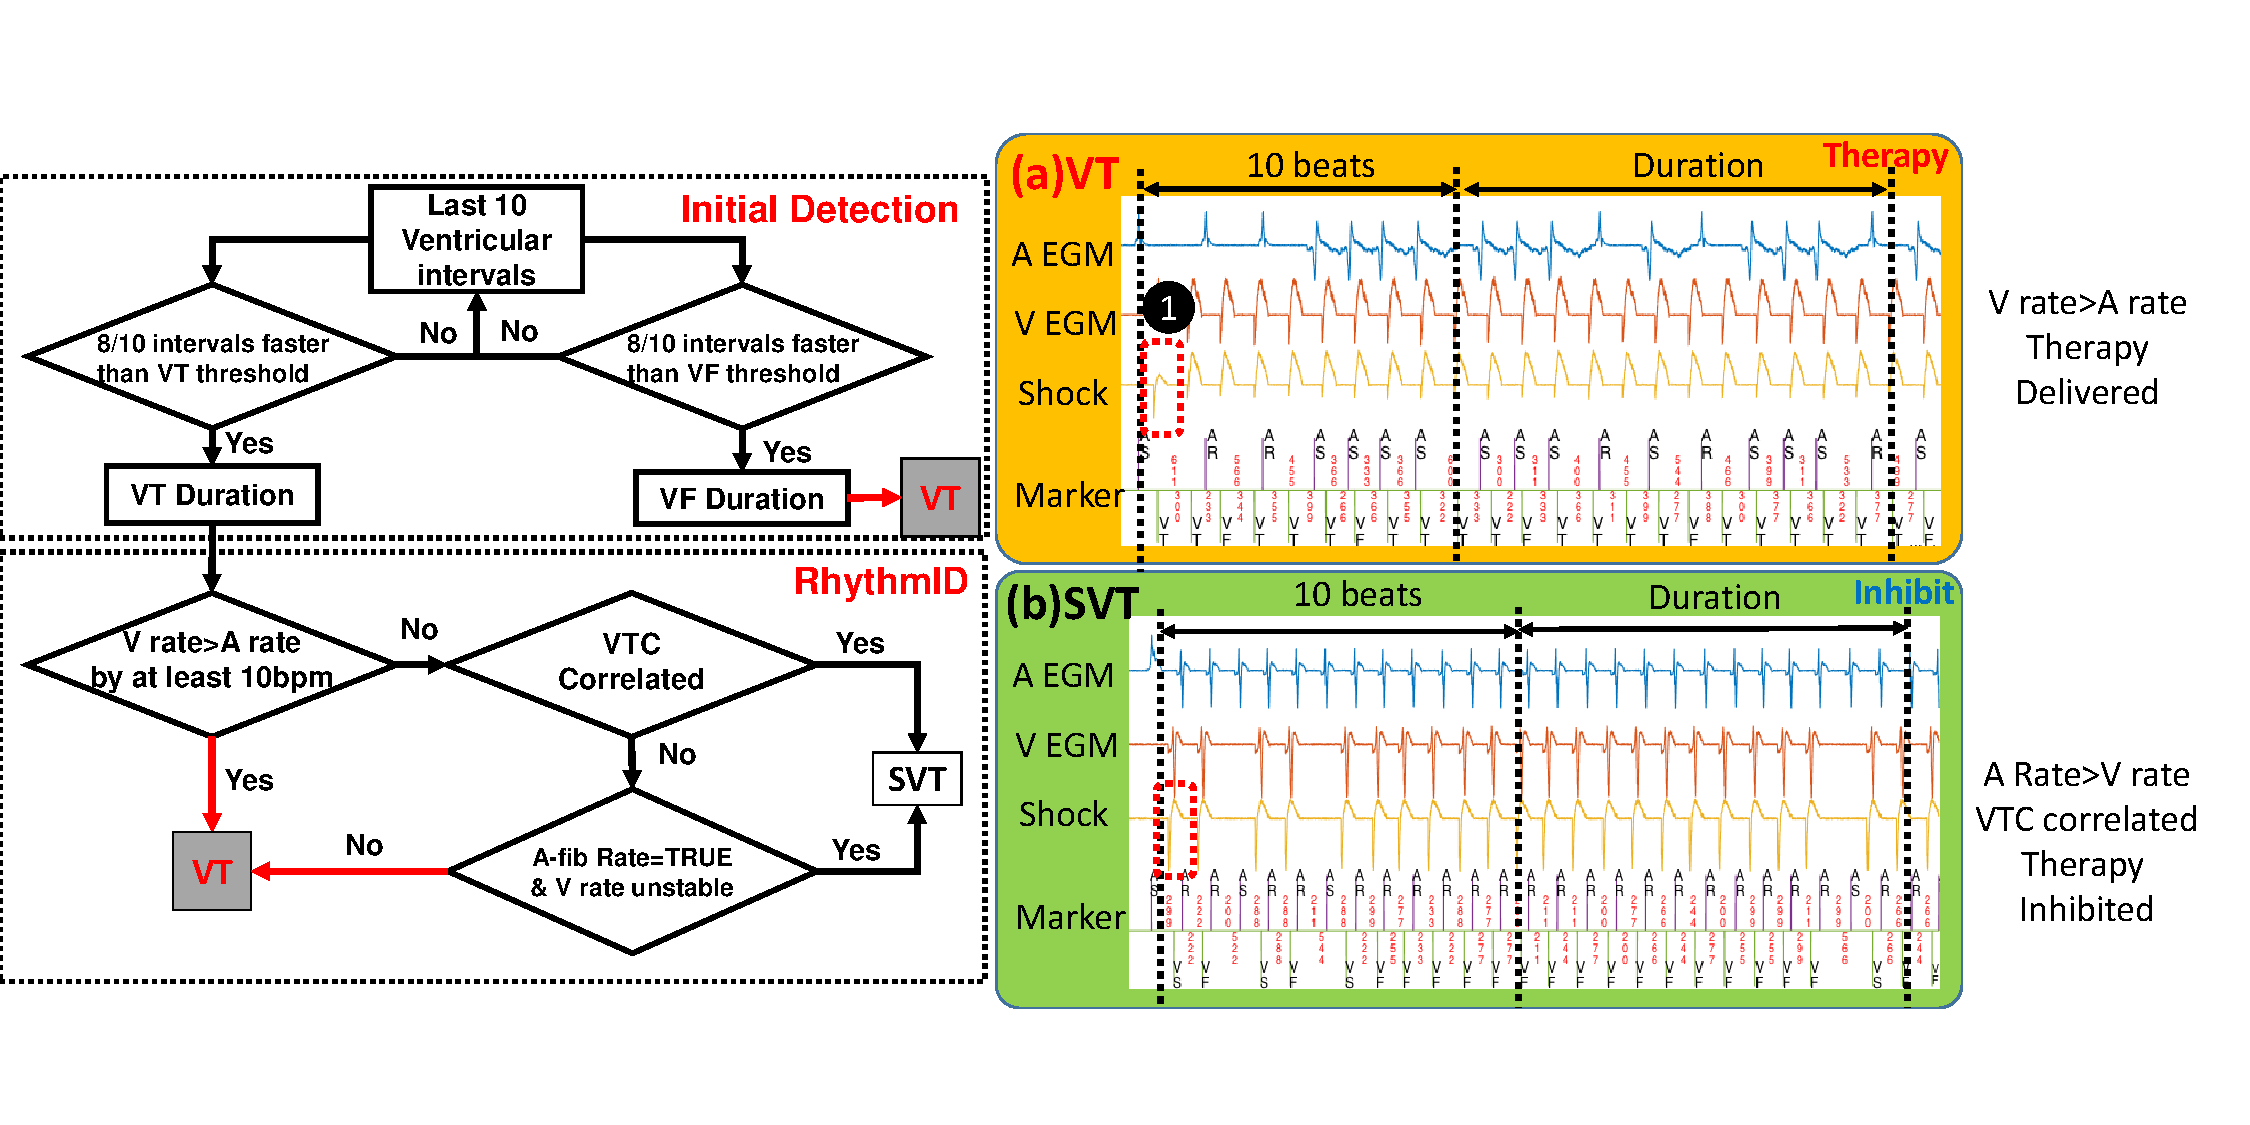
\includegraphics[scale=0.38]{figs/BS_det.pdf}
	\vspace{-10pt}
	\caption{\small SVT/VT detection algorithm by Boston Scientific \cite{compass}. The two cases on the right illustrate two different decisions by the algorithm. (a) illustrates a sustained VT case where at the end of the Duration, the ventricular rate is faster than the atrial rate. The algorithm correctly identified the rhythm as VT and delivered therapy. (b) illustrates a SVT case where at the end of the Duration, the ventricular rate is slower than the atrial rate. Then by comparing the EGM morphology in the Shock channel (Marker 1) with the stored NSR template (Marker 2) for the last 10 EGM events, the algorithm decided that the morphology is correlated, therefore therapy is inhibited.}
	\label{fig:BS_det}
\end{figure*}

\subsubsection{Rhythm ID}
Rhythm ID's decision tree is shown in Fig.~\ref{fig:BS_det}.
Rhythm ID detects an episode by continuously examining the last 10 ventricular intervals and comparing them with VT and VF thresholds. 
If 8/10 intervals are shorter than the VF threshold for a certain pre-set \emph{VF Duration} (e.g., 2.5 seconds) then the algorithm declares VF.
Otherwise, if 8/10 intervals are shorter than the VT threshold for a certain VT Duration, then further discriminators are used.
First, if the ventricular rate is greater than the atrial rate for the last 10 ventricular beats, Rhythm ID will determine the condition is VT.
Otherwise, the Vector Timing and Correlation (VTC) discriminator~\cite{VTC} compares EGM morphology of the last 10 ventricular events with an EGM \emph{template} saved during \ac{NSR}.
VTC is based on the assumption that the EGM morphology of the shock channel during VT is different from its morphology during SVT and NSR.
If the correlation between the current EGM's morphology and the stored NSR morphology is above a pre-set threshold, the current rhythm is more likely to be SVT than VT, and therapy is withheld.
Otherwise, if the atrial rate is equal to a pre-set fibrillation rate and the variance of the ventricular interval length exceeds a certain limit, the algorithm decides it's an \ac{SVT}. 
Otherwise, it decides this is a \ac{VT}.
%As shown in Fig. \ref{fig:BS_det}(b), at the end of the duration, the atrial rate is faster than the ventricular rate. 
%The morphology in the shock channel is similar to the NSR morphology (red dashed) so VTC is correlated and therapy is inhibited.
%As a comparison the morphology during VT is different from the NSR morphology (Marker 1 in Fig. \ref{fig:BS_det}).

\subsubsection{PR Logic+Wavelet}
PRL+W also utilizes rate-based and morphology-based discriminators similar (but not identical) to Rhythm ID.
The morphology discriminator used in PRL+W  is similar to VTC in Rhythm ID, but operates in the wavelet domain~\cite{Wavelet}.
PRL+W also continuously compares the pattern of atrial and ventricular activation to 19 pre-defined patterns~\cite{Singer}.
Each pattern is associated to a heart condition, like Sinus Tachycardia or \ac{VT}.
A match between the current activity and one of the pre-defined patterns is used as an indication that the current rhythm is explained by the associated condition.
